% ===================== SearchAuditBench =====================
\subsection{SearchAuditBench (SearchAuditor)}\label{ds:searchauditbench}
\badgerow{\naturalbadge\ \okbadge\ \lbl{step + span + root cause + repair}\ \lbl{single-agent}\ \lbl{BrowseComp(-ZH) / DeepSearchQA / SEALQA / xBench-DeepSearch}}

\begin{identity}
Paper & \emph{SearchAuditor: Auditing and Attributing Failures in Long-Horizon Search Agents} --- Liang, Liu, Huang, Zhao, Huang, Wang, Duan, Cao (no affiliation on the arXiv page), arXiv:2608.05212, Aug 2026 (preprint, no venue yet) \cite{searchauditor2026}\\
Links & \href{https://github.com/lzzzx666/SearchAuditor}{GitHub \code{lzzzx666/SearchAuditor}} (code, prompts and the data as \code{SearchAuditBench/SearchAuditBench.zip}) \textperiodcentered\ no HF dataset, no project page\\
License & \textbf{none stated} (no LICENSE file); the trajectories embed verbatim search and page returns, and the queries come from BrowseComp, BrowseComp-ZH, DeepSearchQA, Seal-0 and xBench-DeepSearch, whose terms apply\\
Status & downloaded in full, ungated; 390 MB (one 313 MB JSONL); \code{data/searchauditbench/extracted/benchmark\_data\_1243.jsonl}. The ZIP is PPMd-compressed: \code{unzip} and Python's \code{zipfile} fail, 7-Zip is required (the README says so)\\
\end{identity}

\begin{multicols}{2}
\paragraph{Description} SearchAuditBench frames attribution as \emph{trajectory auditing} for deep-search (web research) agents. Given the query, the agent's wrong final answer and the frozen trajectory --- but \emph{no} gold answer and no web access --- an auditor must (1) localise the \textbf{critical error step} (an assistant decision message), (2) classify the \textbf{root cause} into a six-way search-specific taxonomy and (3) write a \textbf{repair directive} that is graded against 3--5 case-specific rubrics. All failures are natural. Eight open-weight models with exposed reasoning --- GLM-5.2, Kimi-K2.6, DeepSeek-V4-Pro, Qwen3.5-397B-A17B and the deep-research specialists OpenSeeker, OpenResearcher, Quest-35B, Tongyi-DeepResearch-30B-A3B --- were run under a single ReAct scaffold adapted from Tongyi DeepResearch with two tools, \code{search} (list of queries) and \code{visit} (URLs + goal), on five benchmarks. 3,500 raw runs $\to$ 3,288 gradable $\to$ 1,674 judged wrong by an LLM evaluator $\to$ after dropping non-auditable cases (evaluator false negatives, flawed items, truncated traces, environment-caused failures, no single critical step) \textbf{1,243 annotated failures}, 125--175 per model. \textbf{Annotation}: four annotators from the author team, each case labelled by \emph{one} of them (disjoint split, so no agreement coefficient exists); Claude Opus 4.6 pre-screens candidate error regions with rationales, humans verify, relocate or relabel, and every field is human-written. The critical step is the earliest decision at which the root-cause mechanism is established; a \textbf{tolerance span} $[k_s,k_e]$ brackets equally defensible adjacent decisions. \textbf{Taxonomy}: \emph{Candidate Mismanagement} (premature lock-in, wrong rejection, failure to converge), \emph{Search Coverage Gap} (decisive evidence path never searched), \emph{Constraint Neglect} (accepts a candidate violating a visible hard constraint), \emph{Unverified Source Reliance} (trusts a snippet or secondary source), \emph{Entity--Relation Misbinding} (right fact, wrong entity/time/slot) and \emph{Unsupported Answer} (residual guess from memory). Rubrics are graded by DeepSeek-V4-Flash, validated against humans (30/713 false passes, 43/159 false fails; paper App.~D).

\paragraph{Metrics and baselines} CS-Strict (exact critical message), CS-Loose (inside the span), RC-Acc / RC-F1 (6-way), Diag = RC correct $\wedge$ CS-Loose, Rep@Diag (all rubrics pass, given Diag) and the end-to-end \textbf{FPS} = Diag $\times$ Rep@Diag. Baselines are Who\&When-style prompting and AgentRx; Claude-Opus-4.8 backbone, \% (paper Table 2):

\begin{center}\small\setlength{\tabcolsep}{3.5pt}
\begin{tabular}{@{}lcccccc@{}}\toprule
Auditor & CS-S & CS-L & RC-Acc & Diag & Rep@D & FPS\\\midrule
All-at-Once & 32.1 & 47.1 & 47.6 & 28.2 & 71.5 & 20.2\\
Step-by-Step & 23.1 & 37.7 & 37.5 & 18.9 & 68.9 & 13.0\\
Binary Search & 32.8 & 47.1 & 43.4 & 25.3 & 70.5 & 17.9\\
AgentRx & 35.4 & 49.7 & 43.0 & 26.7 & 46.4 & 12.4\\
SearchAuditor & \textbf{39.9} & \textbf{54.8} & \textbf{50.7} & \textbf{33.7} & \textbf{73.0} & \textbf{24.6}\\\bottomrule
\end{tabular}
\end{center}
With GPT-5.5 SearchAuditor reaches CS-Strict 44.9 / CS-Loose 58.7 / FPS 32.3 against 39.0 / 51.9 / 26.6 for the best baseline; resuming failed LiveBrowseComp runs from the repaired step raises accuracy (paper Table 4). Even the best auditor localises fewer than half of the critical steps exactly.

\paragraph{Schema} One JSONL object per failed run: \code{index}, \code{model}, \code{dataset} (six tags; \code{BrowseComp English} is a separate tag used only for GLM-5.2), \code{query}, \code{predicted\_answer}, \code{gold\_answer} (QC only, hidden from auditors), \code{trajectory} = OpenAI-style messages with \code{message\_index} (0-based), \code{role} (\code{system} / \code{user} / \code{assistant} / \code{tool}), \code{content}, \code{reasoning\_content} (chain of thought), \code{tool\_calls} [\{\code{tool\_name}, \code{tool\_arguments}, \code{tool\_call\_id}\}], \code{finish\_reason}; labels \code{critical\_step} = \{\code{message\_index}, \code{span\_start\_message\_index}, \code{span\_end\_message\_index}\} (always an assistant message; the span may include tool returns), \code{root\_cause\_primary}, \code{rationale.failure\_rationale}, \code{repair\_directive}, \code{repair\_rubrics} [\{\code{requirement}\}]. No train/test split.
\end{multicols}

\paragraph{Statistics} computed from the downloaded JSONL (the paper's Tables 5--7 agree to within rounding).\par\nobreak\vspace{1pt}
\noindent\begin{minipage}[t]{0.53\linewidth}\vspace{0pt}\small
\fitbox{\begin{tabular}{@{}lr@{}}\toprule
 & All (failed only)\\\midrule
trajectories & 1,243\\
generating models / source benchmarks & 8 / 5 (6 tags)\\
messages (sys + user + asst + tool): mean / median (max) & 73.1 / 43 (404)\\
assistant decision steps: mean / median (max) & 34.3 / 20 (201)\\
tool-return messages: mean / median & 36.7 / 21\\
critical message index (0-based): mean / median (max) & 38.2 / 16 (392)\\
relative critical position: mean / median & 0.58 / 0.58\\
tolerance span (messages): mean / median (min -- max) & 4.3 / 4 (1 -- 12)\\
repair rubrics / instance: mean (range) & 4.4 (3 -- 5)\\
characters / trajectory: mean / median (max) & 209\,k / 123\,k (1.85\,M)\\
query / predicted answer length (chars): median & 146 / 669\\\bottomrule
\end{tabular}}

\smallskip Long tail: 350 runs have $<$20 messages but 202 have $\ge$150. The critical step is the final-answer message in 210 cases (16.9\%) and lies in the last fifth of the run in 420 (33.8\%); by root cause the median relative position is 0.40 for Search Coverage Gap, 0.50 Candidate Mismanagement, 0.59 Unverified Source Reliance, 0.62 Entity--Relation Misbinding, 0.85 Constraint Neglect and 1.0 Unsupported Answer. Tool calls: 32\,k \code{search}, 13.6\,k \code{visit} (a handful of stray names such as \code{web\_search}). Paper-reported token counts: 65.1\,k per trajectory on average (median 39.4\,k, P90 152\,k), of which 49.1\,k are tool returns and 15.3\,k reasoning.
\end{minipage}\hfill
\begin{minipage}[t]{0.45\linewidth}\vspace{0pt}
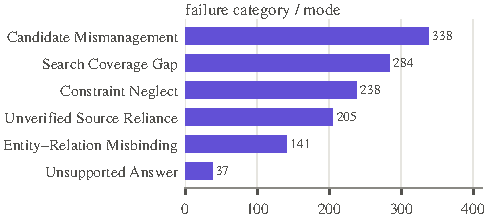
\includegraphics[width=\linewidth]{6_related/searchauditbench/figures/cat.pdf}\\[2pt]
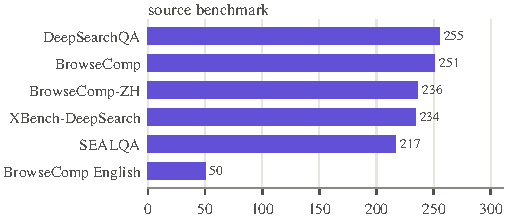
\includegraphics[width=\linewidth]{6_related/searchauditbench/figures/bench.pdf}
\end{minipage}

\paragraph{Example trajectory} \code{index} 546 (GLM-5.2 on xBench-DeepSearch; 8 messages = 3 assistant decisions, 9\,k characters; the shortest run whose critical step is not the final answer). The Chinese query asks where a $>$100\,M-view IShowSpeed short was filmed; after two searches the agent visits a UniFuncs aggregation page, accepts its claim (a pit in Handan, Hebei) and answers, never opening the actual YouTube short --- gold answer Changsha. Label: \emph{Unverified Source Reliance} at message 5, span [5, 7], with rationale, repair directive and four rubrics.
% auto-generated by scripts/render_traj.py -- do not edit
\trajtask{546}{IShowSpeed\cjk{在}YouTube\cjk{上发布过一条关于物理挑战的播放量过亿的短视频（截至}2025\cjk{年}5\cjk{月}18\cjk{日），请问视频是在哪拍摄的？}}
\begin{trajstep}{0}{system}{agA}
Content:\allowbreak{} You are a deep research assistant. Your core function is to conduct thorough,\allowbreak{} multi-source investigations into any topic. You must handle both broad,\allowbreak{} open-domain inquiries and queries within specialized academic fields. For every request,\allowbreak{} synthesize information from credible,\allowbreak{} diverse sources to deliver a comprehensive,\allowbreak{} accurate,\allowbreak{} and objective response. When you have gathered sufficient information and are ready to provide the definitive response,\allowbreak{} you must enclose the entire final answer within <answer></\allowbreak{}answer> tags.\par Current date:\allowbreak{} 2026-06-23
\end{trajstep}
\begin{trajstep}{1}{user}{agB}
Content:\allowbreak{} IShowSpeed\cjk{在}YouTube\cjk{上发布过一条关于物理挑战的播放量过亿的短视频（截至}2025\cjk{年}5\cjk{月}18\cjk{日），请问视频是在哪拍摄的？}
\end{trajstep}
\begin{trajstep}{2}{assistant}{agC}
Thought:\allowbreak{} The user is asking about an IShowSpeed YouTube short video about a physical challenge that has over 100 million views (as of May 18,\allowbreak{} 2025),\allowbreak{} and where it was filmed. Let me search for this.\newline Action (tool\_calls):\allowbreak{} [\{"tool\_name":\allowbreak{} "search",\allowbreak{} "tool\_arguments":\allowbreak{} \{"query":\allowbreak{} "IShowSpeed YouTube short 100 million views physical challenge"\},\allowbreak{} "tool\_call\_id":\allowbreak{} "chatcmpl-tool-8a2b15e24f33c7c4"\},\allowbreak{} \{"tool\_name":\allowbreak{} "search",\allowbreak{} "tool\_arguments":\allowbreak{} \{"query":\allowbreak{} "IShowSpeed \cjk{播放量过亿} \cjk{短视频} \cjk{物理挑战}"\},\allowbreak{} "tool\_call\_id":\allowbreak{} "chatcmpl-tool-aec006d5a75e3a55"\}]
\end{trajstep}
\begin{trajstep}{3}{tool (search)}{agD}
Observation (tool return):\allowbreak{} A Google search for 'IShowSpeed YouTube short 100 million views physical challenge' found 10 results:\allowbreak{}\par \#\# Web Results\newline 1. [\$100000 WIPEOUT with MrBeast and KSI - IShowSpeed - YouTube](https:\allowbreak{}/\allowbreak{}/\allowbreak{}www.youtube.com/\allowbreak{}watch?\allowbreak{}v=\allowbreak{}iitET2IZ0rE)\newline Date published:\allowbreak{} Jun 4,\allowbreak{} 2024\newline for tips/\allowbreak{}donations text to speech is here :\allowbreak{} https:\allowbreak{}/\allowbreak{}/\allowbreak{}streamlabs.com/\allowbreak{}ishowspeed/\allowbreak{}tip Media request for your video to pop up is here ...\par 2. [IShowSpeed Celebrates 40 Million Subscribers with Jump - TikTok](https:\allowbreak{}/\allowbreak{}/\allowbreak{}www.tiktok.com/\allowbreak{}@espn/\allowbreak{}video/\allowbreak{}7512857117418736926?\allowbreak{}lang=\allowbreak{}en)\newline Date published:\allowbreak{} Jun 6,\allowbreak{} 2025\newline Watch IShowSpeed's epic reaction as he hits 27 million subscribers on\newline [...] (2,\allowbreak{}076 chars omitted) [...]\newline yahoo.com/\allowbreak{}entertainment/\allowbreak{}articles/\allowbreak{}ishowspeed-takes-50-push-ups-180850976.html)\newline Date published:\allowbreak{} Nov 11,\allowbreak{} 2025\newline During a recently conducted livestream,\allowbreak{} the popular streamer surprised his fans by doing 50 push-ups in front of the camera,\allowbreak{} just to disprove ...
\end{trajstep}
\begin{trajstep}{4}{tool (search)}{agD}
Observation (tool return):\allowbreak{} A Google search for 'IShowSpeed \cjk{播放量过亿} \cjk{短视频} \cjk{物理挑战}' found 10 results:\allowbreak{}\par \#\# Web Results\newline 1. [IShowSpeed\cjk{亿级视频拍摄地揭秘}- U\cjk{深搜} - UniFuncs](https:\allowbreak{}/\allowbreak{}/\allowbreak{}unifuncs.com/\allowbreak{}s/\allowbreak{}PSEtt1XB)\newline IShowSpeed\cjk{在}YouTube\cjk{上发布的物理挑战视频拍摄于中国河北省邯郸市永年区洺珠小镇的八卦坑。该视频拍摄于}2025\cjk{年}4\cjk{月初，内容为}IShowSpeed\cjk{在一个彩色锥形坑中通过螺旋奔跑} ...\par 2. [ishowspeed youtube \cjk{物理挑战播放量过亿短视频拍摄地点的相關文章}](https:\allowbreak{}/\allowbreak{}/\allowbreak{}www.juksy.com/\allowbreak{}tag/\allowbreak{}ishowspeed\%20youtube\%20\%E7\%89\%A9\%E7\%90\%86\%E6\%8C\%91\%E6\%88\%98\%20\%E6\%92\%AD\%E6\%94\%BE\%E9\%87\%8F\%E8\%BF\%87\%E4\%BA\%BF\%20\%E7\%9F\%AD\%E8\%A7\%86\%E9\%A2\%91\%20\%E6\%8B\%8D\%E6\%91\%84\%E5\%9C\%B0\%E7\%82\%B9)\newline \cjk{探索}JUKSY \cjk{街星上}\#ishowspeed youtube \cjk{物理挑战播放量过亿短视频拍摄地点標籤下的}1 \cjk{篇精選文章，涵蓋最新時尚潮流、生活風格與娛樂情報。}\par 3. [Speed takes on the physics chal\newline [...] (2,\allowbreak{}598 chars omitted) [...]\newline /\allowbreak{}ishowspeed\%20\%E7\%89\%A9\%E7\%90\%86\%E6\%8C\%91\%E6\%88\%98\%20\%E7\%9F\%AD\%E8\%A7\%86\%E9\%A2\%91\%20\%E8\%BF\%87\%E4\%BA\%BF\%20\%E6\%92\%AD\%E6\%94\%BE\%E9\%87\%8F)\newline \cjk{甲亢哥}IShowSpeed WWE \cjk{摔角狂熱}42 \cjk{迎首秀！頂繩飛身重擊}Logan Paul \cjk{砸穿播報桌！} WWE \cjk{摔角狂熱}42\cjk{（}WrestleMania 42\cjk{）於}2026 \cjk{年}4 \cjk{月}18 \cjk{日在拉斯維加斯忠實體育場（}Allegiant ...
\end{trajstep}
\begin{faultystep}{5}{assistant}{agC}
Thought:\allowbreak{} The first search result from UniFuncs seems to have the answer. Let me visit that page to confirm.\newline Action (tool\_calls):\allowbreak{} [\{"tool\_name":\allowbreak{} "visit",\allowbreak{} "tool\_arguments":\allowbreak{} \{"goal":\allowbreak{} "\cjk{确认}IShowSpeed\cjk{物理挑战短视频的拍摄地点}",\allowbreak{} "url":\allowbreak{} ["https:\allowbreak{}/\allowbreak{}/\allowbreak{}unifuncs.com/\allowbreak{}s/\allowbreak{}PSEtt1XB"]\},\allowbreak{} "tool\_call\_id":\allowbreak{} "chatcmpl-tool-ab2de3fc9ef44113"\}]
\end{faultystep}
\begin{trajstep}{6}{tool (visit)}{agE}
Observation (tool return):\allowbreak{} The useful information in https:\allowbreak{}/\allowbreak{}/\allowbreak{}unifuncs.com/\allowbreak{}s/\allowbreak{}PSEtt1XB for user goal \cjk{确认}IShowSpeed\cjk{物理挑战短视频的拍摄地点} as follows:\allowbreak{}\par Evidence in page:\allowbreak{}\newline \cjk{根据多个可靠来源的交叉验证，}IShowSpeed\cjk{在}YouTube\cjk{上发布的物理挑战视频拍摄地点是：}\par \#\#\# \cjk{具体位置}\par **\cjk{河北省邯郸市永年区洺珠小镇的八卦坑}** \cjk{（也称}"\cjk{太极八卦坑}"\cjk{或}"\cjk{洺珠八卦坑}"\cjk{）}\par \#\#\# \cjk{详细地址信息}\par * **\cjk{国家}** \cjk{：中国}\newline * **\cjk{省份}** \cjk{：河北省}\newline * **\cjk{城市}** \cjk{：邯郸市}\newline * **\cjk{区县}** \cjk{：永年区}\newline * **\cjk{具体地点}** \cjk{：洺珠小镇（洺珠酷跳健身园）}\newline * **\cjk{景点名称}** \cjk{：八卦坑} /\allowbreak{} \cjk{太极八卦坑}\par \#\#\# \cjk{视频内容背景}\par IShowSpeed\cjk{在该景点进行了}"\cjk{物理挑战}"\cjk{，需要在一个彩色的锥形坑中通过螺旋奔跑的方式利用离心力从坑底上升到顶部，成功逃离坑底。这是一个网红打卡的游乐项目，难度较高，不少网络红人都曾挑战过。}\par \#\#\# \cjk{拍摄时间}\par \cjk{该视频拍摄于}2025\cjk{年}IShowSpeed\cjk{中国行期间，具体时间是}2025\cjk{年}4\cjk{月初（}Instagram\cjk{发布时间为}2025\cjk{年}4\cjk{月}9\cjk{日）。}\par \#\#\# \cjk{多源验证}\par \cjk{我通过多个独立来源验证了这一信息：}\par * Instagram\cjk{上的多个帖子明确提到}"IShowSpeed\cjk{來到河北邯鄲}\newline [...] (57 chars omitted) [...]\newline he Eight Diagrams Pit (Bagua Keng),\allowbreak{} In Handan City,\allowbreak{} Hebei Province,\allowbreak{} Mainland China"\par Summary:\allowbreak{}\newline \cjk{根据网页内容中多轮搜索和交叉验证的结果，}IShowSpeed\cjk{的物理挑战短视频拍摄于中国河北省邯郸市永年区洺珠小镇的八卦坑（也称太极八卦坑）。该视频拍摄于}2025\cjk{年}4\cjk{月，内容为挑战从彩色锥形坑底部利用离心力螺旋奔跑至顶部。此结论得到了}Instagram\cjk{、抖音、}TikTok\cjk{等多个独立来源的一致确认，信息可靠性高。}
\end{trajstep}
\begin{trajstep}{7}{assistant}{agC}
Thought:\allowbreak{} \cjk{我已经得到了答案。}\newline Content:\allowbreak{} <answer>\par IShowSpeed \cjk{在} YouTube \cjk{上发布的那条播放量过亿的物理挑战短视频，拍摄地点是}**\cjk{中国河北省邯郸市永年区洺珠小镇的}"\cjk{八卦坑}"**\cjk{（也称}"\cjk{太极八卦坑}"\cjk{）。}\par **\cjk{具体信息：}**\par - **\cjk{地点}**\cjk{：河北省邯郸市永年区洺珠小镇（洺珠酷跳健身园）内的八卦坑景点}\newline - **\cjk{拍摄时间}**\cjk{：}2025 \cjk{年} 4 \cjk{月初（}IShowSpeed \cjk{中国行期间）}\newline - **\cjk{视频内容}**\cjk{：}IShowSpeed \cjk{在一个彩色锥形坑中，通过螺旋奔跑的方式利用离心力从坑底上升到顶部，完成}"\cjk{物理挑战}"\cjk{逃脱。这是一个网红打卡游乐项目，难度较高。}\par \cjk{该结论得到了} Instagram\cjk{、抖音、}TikTok \cjk{等多个独立来源的交叉验证。}\par </\allowbreak{}answer>
\end{trajstep}
\trajannotation{assistant (single search agent)}{5}{Unverified Source Reliance}{The decisive error occurs at message 5,\allowbreak{} where the agent treats a UniFuncs aggregation page as the confirming evidence after seeing a direct YouTube short result and the IShowSpeed channel in search results. The trajectory never opens or verifies the exact IShowSpeed YouTube short,\allowbreak{} does not check the dated view-count threshold,\allowbreak{} and does not prove that the location evidence belongs to the same qualifying video rather than a repost or similar physics challenge clip. The final location therefore depends on an unverified secondary summary rather than primary or reliably corroborated evidence.}{\cjk{长沙}}{<answer>\par IShowSpeed \cjk{在} YouTube \cjk{上发布的那条播放量过亿的物理挑战短视频，拍摄地点是}**\cjk{中国河北省邯郸市永年区洺珠小镇的}"\cjk{八卦坑}"**\cjk{（也称}"\cjk{太极八卦坑}"\cjk{）。}\par **\cjk{具体信息：}**\par - **\cjk{地点}**\cjk{：河北省邯郸市永年区洺珠小镇（洺珠酷跳健身园）内的八卦坑景点}\newline - **\cjk{拍摄时间}**\cjk{：}2025 \cjk{年} 4 \cjk{月初（}IShowSpeed \cjk{中国行期间）}\newline -\newline [...] (63 chars omitted) [...]\newline \cjk{脱。这是一个网红打卡游乐项目，难度较高。}\par \cjk{该结论得到了} Instagram\cjk{、抖音、}TikTok \cjk{等多个独立来源的交叉验证。}\par </\allowbreak{}answer>}{\textbf{tolerance\_span}: [5,\allowbreak{} 7]; \textbf{repair\_directive}: Return to source verification. Open or reliably archive the exact IShowSpeed YouTube short or channel result,\allowbreak{} verify that it is the physical-challenge video and that it met the requested view threshold by the specified date,\allowbreak{} then corroborate the filming location for that same video using primary metadata,\allowbreak{} original description,\allowbreak{} credible reporting,\allowbreak{} or verifiab\newline [...] (3 chars omitted) [...]\newline visual/\allowbreak{}location evidence. Do not accept an aggregation page or social snippet unless it is independently tied to the exact qualifying video.; \textbf{repair\_rubrics}: [\{"requirement":\allowbreak{} "A valid repair must verify the exact YouTube short or channel posting rather than relying on an aggregation page."\},\allowbreak{} \{"requirement":\allowbreak{} "A valid repair must check that the same video satisfies the physical-challenge description and the dated view-count threshold."\},\allowbreak{} \{"requirement":\allowbreak{} "A valid repair must bind filming-location evidence to the exa\newline [...] (106 chars omitted) [...]\newline epair must use primary metadata,\allowbreak{} credible reporting,\allowbreak{} or independently verifiable visual/\allowbreak{}location evidence before finalizing the location."\}]; \textbf{model}: GLM-5.2; \textbf{source\_benchmark}: XBench-DeepSearch}


\paragraph{Notes} (i) Richest label set in the survey: critical step \emph{with tolerance span}, root cause, rationale, repair directive \emph{and} executable rubrics --- the only dataset that scores ``how to fix'' (diagnosis-gated repair grading), so it is the natural test-bed for attribution-to-repair pipelines. (ii) Long and evidence-heavy: tool returns are stored verbatim (median 123\,k, max 1.85\,M characters), and the set is multilingual --- BrowseComp-ZH queries plus several models reasoning in Chinese even on English benchmarks. (iii) Label provenance: one author-team annotator per case after a Claude Opus 4.6 pre-screen; no inter-annotator agreement is reported, and the authors note the pre-screening model is deliberately absent from the evaluated auditors. (iv) Positional skew: a third of critical steps fall in the last 20\% and Constraint Neglect / Unsupported Answer are late by construction, so ``blame the last assistant step'' is a non-trivial CS-Loose baseline. (v) One scaffold, one role: all eight models share the same \code{search}/\code{visit} loop, so there is no framework or agent-level variation to attribute to; no license and no official split. (vi) Overlaps: BrowseComp queries also underlie AgentErrata's injected failures, and AgentRx is used here as a baseline, but no trajectories are shared.
